\documentclass[12pt,fleqn]{exam}
\usepackage{pifont}
\usepackage{dingbat}
\usepackage{amsmath,amssymb}
\usepackage{epsfig}
\usepackage[colorlinks=true,linkcolor=black,anchorcolor=black,citecolor=black,filecolor=black,menucolor=black,runcolor=black,urlcolor=black]{hyperref}
\usepackage[letterpaper, margin=0.75in]{geometry}
\addpoints
\boxedpoints
\pointsinmargin
\pointname{pts}

\usepackage[activate={true,nocompatibility},final,tracking=true,kerning=true,factor=1100,stretch=10,shrink=10]{microtype}
\usepackage[american]{babel}
%\usepackage[T1]{fontenc}
\usepackage{fourier}
\usepackage{isomath}
\usepackage{upgreek,amsmath}
\usepackage{amssymb}

\newcommand{\dotprod}{\, {\scriptzcriptztyle
    \stackrel{\bullet}{{}}}\,}

\newcommand{\reals}{\mathbf{R}}
\newcommand{\lub}{\mathrm{lub}} 
\newcommand{\glb}{\mathrm{glb}} 
\newcommand{\complex}{\mathbf{C}}
\newcommand{\dom}{\mbox{dom}}
\newcommand{\range}{\mbox{range}}
\newcommand{\cover}{{\mathcal C}}
\newcommand{\integers}{\mathbf{Z}}
\newcommand{\vi}{\, \mathbf{i}}
\newcommand{\vj}{\, \mathbf{j}}
\newcommand{\vk}{\, \mathbf{k}}
\newcommand{\bi}{\, \mathbf{i}}
\newcommand{\bj}{\, \mathbf{j}}
\newcommand{\bk}{\, \mathbf{k}}
\DeclareMathOperator{\Arg}{\mathrm{Arg}}
\DeclareMathOperator{\Ln}{\mathrm{Ln}}
\newcommand{\imag}{\, \mathrm{i}}

\usepackage{graphicx}
\newcommand\AM{{\sc am}}
\newcommand\PM{{\sc pm}}
     
\newcommand{\quiz}{1}
\newcommand{\term}{Fall}
\newcommand{\due}{Wednesday 24 at 13:15 \PM}
\newcommand{\class}{MATH 115}
\begin{document}
\large
\vspace{0.1in}
\noindent\makebox[3.0truein][l]{\textbf{\class}}
\textbf{Name:} \hrulefill \\
\noindent \makebox[3.0truein][l]{\textbf{In class work \quiz, \term \/ \the\year}}
\textbf{Row and Seat}:\hrulefill\\
\vspace{0.1in}


\noindent  In class work  \quiz\/  has questions 1 through  \numquestions \/ with a total of  \numpoints\/  points.   
Digitize your work and submit it to Canvas. This assignment is due \emph{\due}.

\vspace{0.1in}


\begin{questions} 

\question[5] Find the \emph{natural domain} of the function $F$ whose
formula is $F(x) = \frac{1}{5+ \frac{1}{x}}$
\begin{solution}[2.5in]
\end{solution}

\question[5] Use desmos to graph $y = \frac{1}{5+ \frac{1}{x}}$. As 
best you can, reproduce the graph here.  Also, use the graph to determine $\range(F)$.
Be careful! Is one in the range? 
\begin{solution}[2.5in]
\end{solution}


\question Define functions $F(x)= x^2-1$ and $G(x) = 1-x$. Find the
numerical values of 
\begin{parts}
\part $(F+G)(4) = $
\begin{solution}[0.25in]
\end{solution}

\part $(F \circ G)(4) = $
\begin{solution}[0.25in]
\end{solution}

\part $(G \circ F)(4) = $
\begin{solution}[0.25in]
\end{solution}


\end{parts}

\question [5] Show below is a graph of a function $Q$. Given that the
 graph of $Q$ is a translation of the graph of $y=|x|$, what is the formula
 for $Q$?

 \vspace{0.1in}
 \begin{center}
 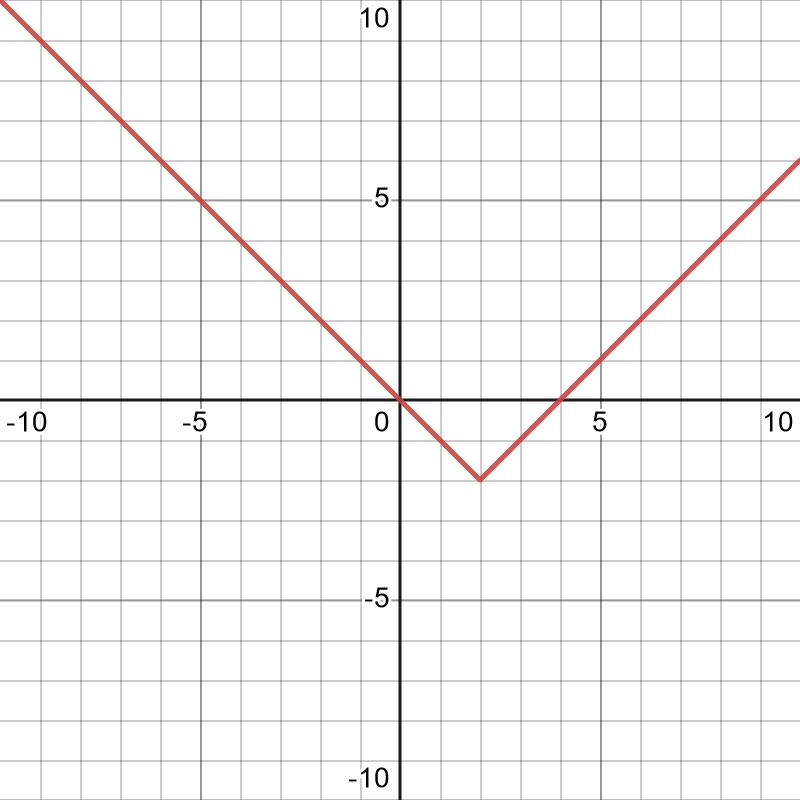
\includegraphics[scale=0.25]{desmos-graph(24).png}
 \end{center}
 
\end{questions}



\end{document}